\subsection{Robotbevægelse ved påføring af speckle patterns} \label{Robotbevægelse ved påføring af speckle patterns}

% Bevægelses mønster
Valget af bevægelsestype for robotten afhænger af, om robotten skal være i kontakt med objektet for at påføre mønstret, eller om den vil kunne påføre mønstret på afstand som ved spraymaling. Alt efter hvilken fremgang, der anvendes kræves der forskellige frihedsgrader, samt forskellige bevægelsesmønstre. Begge disse parameter afhænger af typerne af led der afvendes, i kombination med, hvordan leddene arbejder sammen.


% Joint(led) typer
Der er fire typer af led som alment bruges og de kan opdeles i en lineær gruppe og en rotations gruppe. To af ledtyperne er lineære led og glidende led, som muliggøre bevægelse på en akse. De to andre led er rotationsled og kugleled. Rotationsled muliggør rotation om et punkt i et plan, og udfører derved bevægelser på to akser, ved at rotere om en tredje akse, se figur \ref{fig:rotation i planet}. Kugleled muliggør bevægelse på tre separate akser, hvilket betyder, at der er tale om 3D bevægelser. Kugleled har derigennem også muligheden for, at fungere som rotationsled, ved ikke at bevæge sig på den tredje akse \parencite{Niku2020IntroductionApplications}. Sammensætninger af led typer kan ses på \ref{fig: Sammensætniger af led}.

\begin{figure} [H]
    \centering
    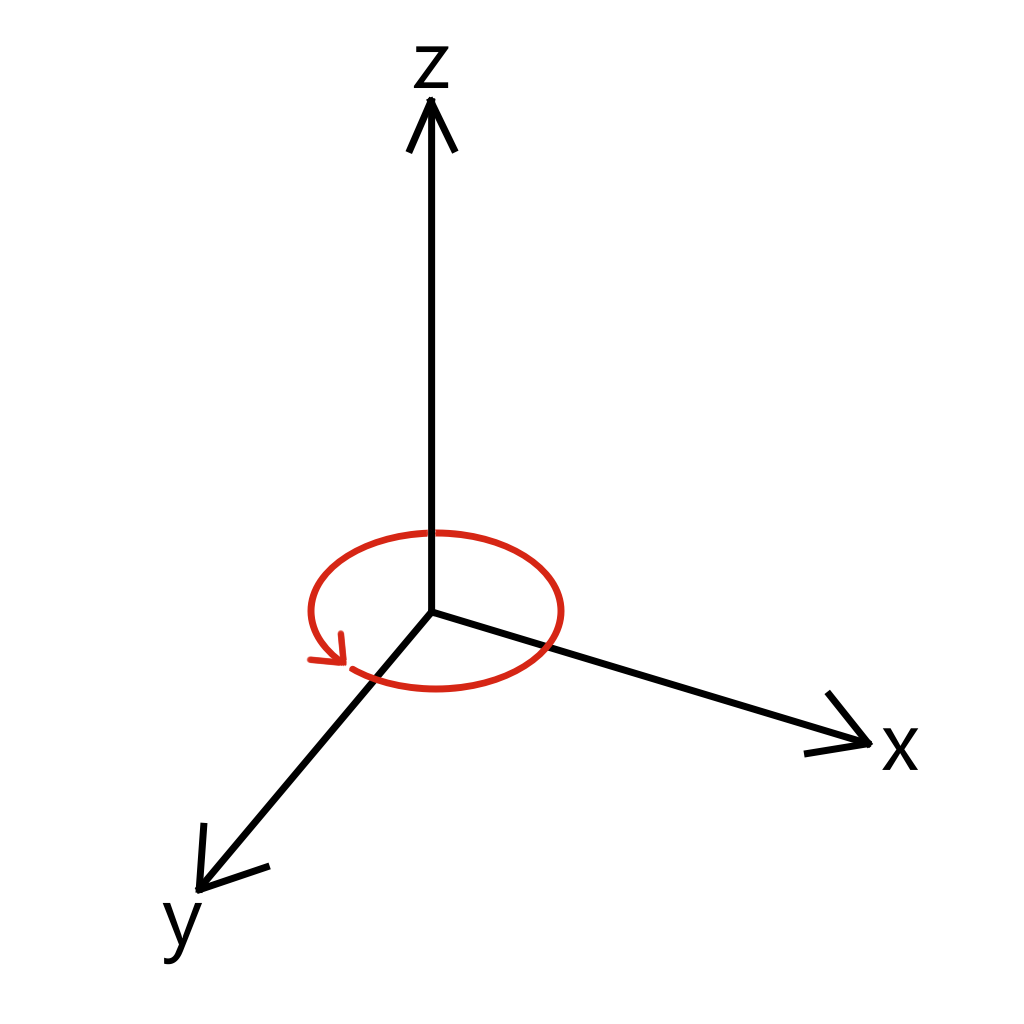
\includegraphics[width=0.4\linewidth]{Sections/2 Problemanalyse/Media/Rotation i planet.png}
    \caption{Illustration af rotation i et xy-plan, omkring z-aksen.}
    \label{fig:rotation i planet}
\end{figure} \plainbreak{-0.5}
% Degree of freedom(on/off)

De forskellige ledtyper giver forskellige mængder af frihedsgrader, hvilket er en angivelse af bevægelsesmulighederne for en robot. Desto større mængde af frihedsgrader, desto mere komplekse bevægelser kan en robot udføre. Dette betyder også, at mængden af bevægelsesudregninger øges i takt med at frihedsgraden stiger. Hvert led har en frihedsgrads værdi, som angiver hvor mange akser leddet kan bevæge sig på eller rotere omkring. Ved tilfælde hvor bevægelsen kun kan være binære, som ved en skinne der er skubbet helt ud eller slet ikke skubbet ud, angives der en halv frihedsgrad. Den totale sum af alle leds frihedsgrader er en robots frihedsgradsværdi.


\begin{figure} [H]
    \centering
    \includegraphics[width=1\linewidth]{Sections/2 Problemanalyse/Media/bevægelse.png}
    \caption{Eksempler på sammensætninger af led, der giver anledning til forskellige bevægelses mønster og frihedsgrader. Billedet er fra \parencite{Niku2020IntroductionApplications}.}
    \label{fig: Sammensætniger af led}
\end{figure} \plainbreak{-0.5}

% Kalibering(waypoints)
For at robotten har en forståelse af hvor emnet er og hvor en bevægelse vil placere robotten, kan der gøres brug af to forskellige tilgange. Den første gør brug af sensorobservation, der gennem inputs klargører hvordan verden ser ud, som nævnt tidligere i dette afsnit. I den anden tilgang forklares robotten, hvordan verden omkring den ser ud. Dette gøres ved softwarerepræsentation, manuel kalibrering eller en kombination. Manuel kalibrering er en udbredt metode hvis en specifik bane ønskes. Der fastlægges stoppunkter, hvilket er et sæt koordinater robotten bruger som reference, ved at manuelt styre robotten til de ønskede referencepunkter.

De to tilgange vil begge kunne anvendes hver for sig, men vil også kunne kombineres for, at gøre brug af, deres forskellige fordele. Eksempelvis produktions- og pakkeriindustrirobotter gør brug af forklaringsmetoden til at udføre deres arbejde, og anvender sensormetoden til at sørge for sikkerhed, i områder, hvor der kan være tale om en dynamisk arbejdsplads.


% Typer af koordinater 
Hvordan en robot kommer fra a til b, spiller en stor rolle, da der kan forekomme fysiske begrænsninger, i form af robottens dele og led, samt der kan være behov for at skulle bevæge sig uden om et fysik objekt. Til planlægningen af en robots bane er der to overordnede tilgange, som kan bruges hver for sig eller kombineres. De to tilgange er henholdsvis arbejdes-domæne, ofte henvist til som kartesiske koordinater, og led-domæne \parencite{Castro2019TrajectoryManipulators}. Led-domæne gør brug af stoppunkter, som en liste af punkter der skal passeres igennem, ud fra punkterne opdeles den påkrævede bevægelse i mindre dele, hvilket er det, der giver anledning til en jævn bevægelse.

Led-domæne kræver færre computerberegninger end kartesiske koordinater og er derved knap så energiintens en metode, grundet den ikke er begrænset af at skulle beregne en bestemt bane, men blot skal nå stoppunkterne. Den jævne bevægelse af leddene betyder der anvendes den mindste bevægelse, der kræves for at nå stoppunkterne. Dette betyder dog, som nævnt, at der ikke er kontrol over banen derhen.

Ved arbejdes-domæne tilgangen gøres der brug af koordinat systemer til at fastlægge positionen af hvert enkelet led. Der vil dertil være et låst koordinatsystem, som også kaldes det globale system, hvilket tilsvarer området robotten befinder sig i. Derudover har de forskellige led hver deres koordinatsystem, som kaldes lokal systemer. Disse lokal systemer flytter sig med de enkelte led og anvender det globale system som reference \parencite{Castro2019TrajectoryManipulators}. Se figur \ref{fig:Global og lokal systemer}.

\begin{figure} [H]
    \centering
    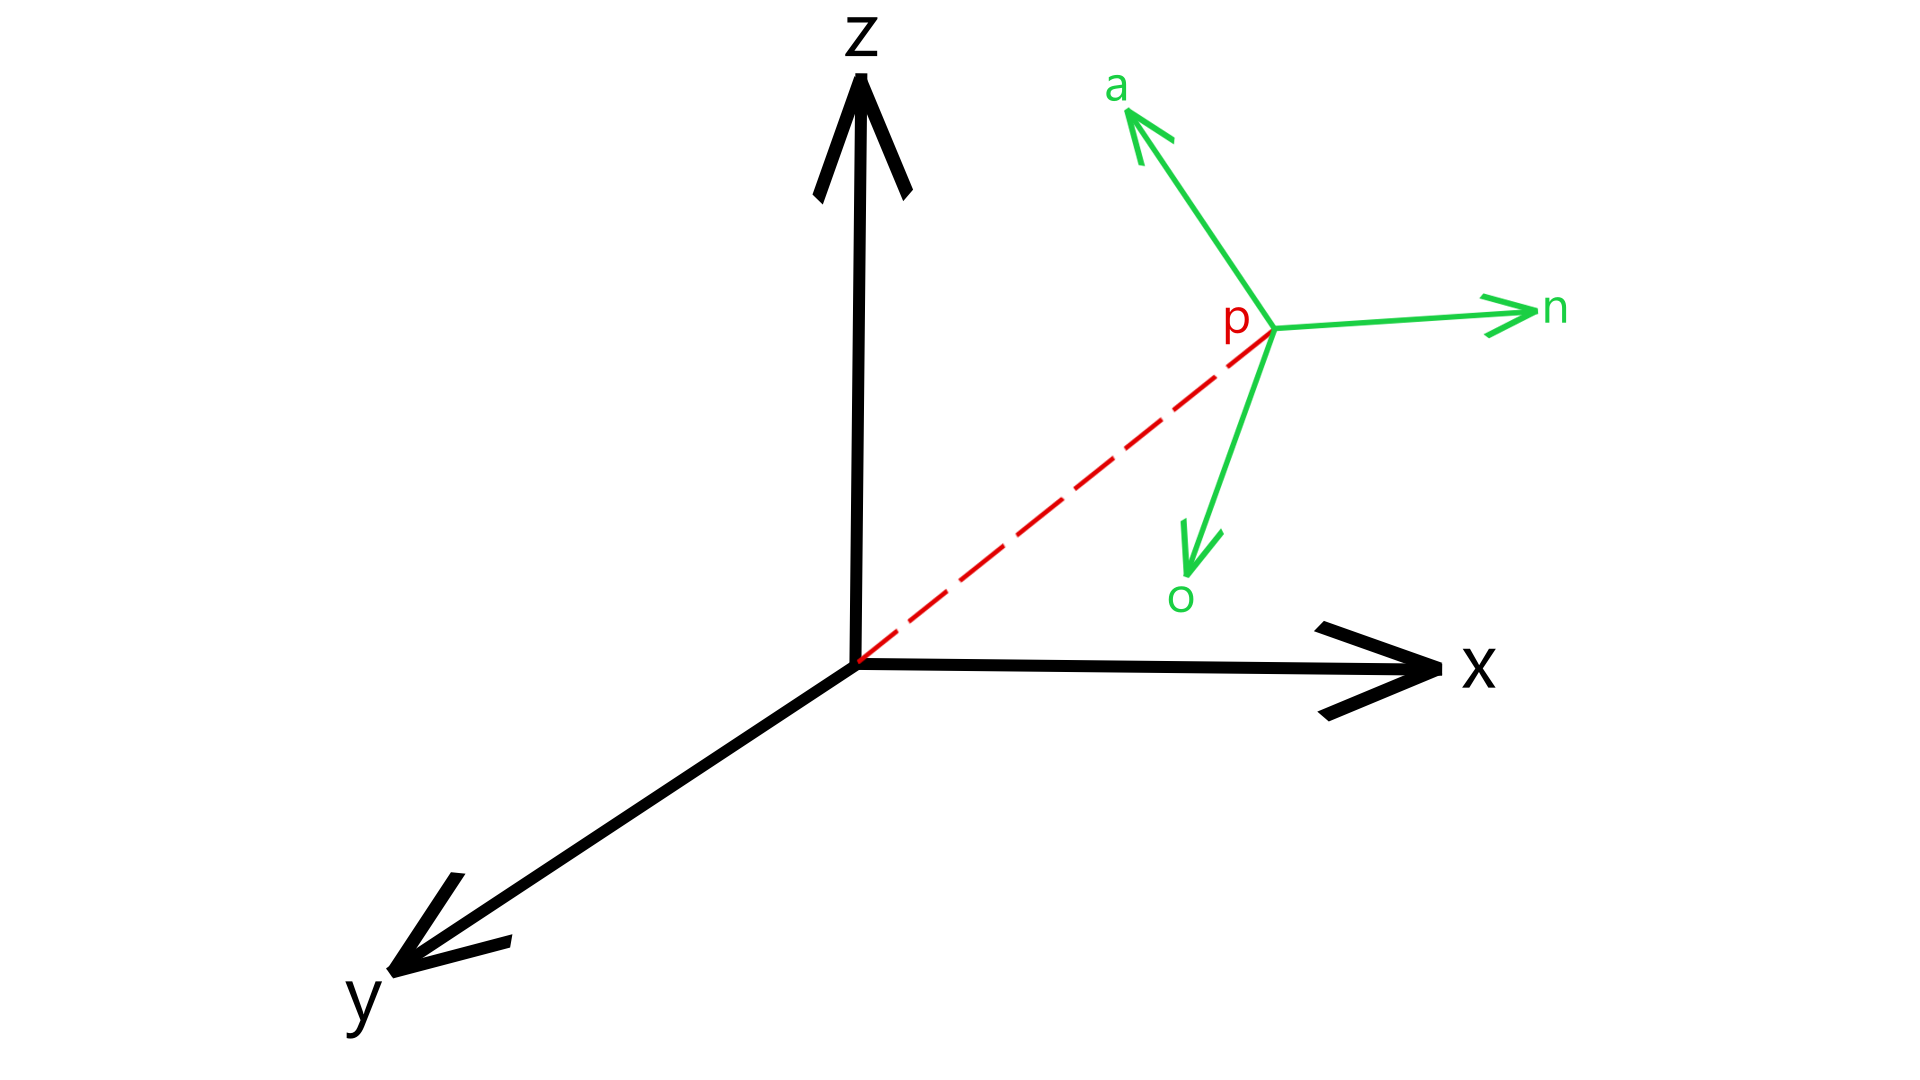
\includegraphics[width=0.7\linewidth]{Sections/2 Problemanalyse/Media/Global og local frames.png}
    \caption{Illustration af global og lokal systemer. De sort akser er det globale system, de grønne akser er et lokal system der tilhøre punktet p. Punktet p repræsenterer et led.}
    \label{fig:Global og lokal systemer}
\end{figure} \plainbreak{-0.5}

% IK
Alt efter om robottens led opererer separat eller påvirker de andre leds postion, sker navigation i disse systemer, enten ved at hvert led refererer til det globale system eller ved Invers Kinematik (IK). IK anvender positionen af det sidste/yderste led af en robot, til at fastlægge positioner for de forrige led. Dette kan sammenlignes med en hånd, der skal nå en kaffekop, hvortil albuen og skulderens bevægelser,  fastlægges ud fra hvor hånden skal ende med at være. Dette betyder, at banen bliver fastlagt ud fra, hvordan det sidste led tilbagelægger den mindste mulige strækning. For at ændre denne bane, kan der i strækningerne mellem to stoppunkter tilføjes yderligere punkter, som robotten skal gennemløbe. Ved at justere disse tilføjede punkter, kan banen derved justeres efter behov. For at opnå bevægelse langs eller omkring robotters led, anvendes der aktuatorer. Der anvendes primært tre forskellige typer af aktuatorer, i form af hydrauliske aktuatorer, pneumatiske aktuatorer og elmotorer \parencite{Niku2020IntroductionApplications}.



% Drivkraft
% Hydraulisk aktuator, pneumatisk aktuator & el-motorer
\textbf{Hydrauliske systemer} gør brug af inkompressible væsker og dermed kan overføres kræfter, ved at påvirke væsken med et tryk. Der gælder for hydrauliske systemer at desto større tryk, desto større kraft vil væsken overføre. Forholdet mellem trykforøgningen og forøgelsen af kraften der overføres, følger et tilnærmelsesvis proportionelt forhold. Dette betyder at hydrauliske systemer kan udføre opgaver med god præcision.

Hydrauliske systemer kan operere med højt tryk, i kombination med at den trykgenerende mekanisme ikke behøver at være monteret på robottens bevægelige dele, betyder dette, at de er velegnet til operationer, hvor der skal flyttes tungt gods eller vægten af robottens bevægelige dele skal være minimal. Hydrauliske systemer har derigennem det bedste energi per vægt forhold, men kræver ofte mere vedligeholdelse end andre aktuatormuligheder. \parencite{Niku2020IntroductionApplications}

\textbf{Elmotorer} egner sig, ligesom hydrauliske systemer, godt til præcision, samt kan anskaffes i et bredt spænd af forskellige størrelser og opbygninger \parencite{Kakoty2024IntroductionRobotics}. En elmotor vejer mere end et tilsvarende hydralisk system, da den kraftgenerende del sidder på armen, derfor skal motoren både flytte på armen og sig selv, istedet for blot armen. Fordelen er at der kræves minimal vedligeholdelse.

\textbf{Pneumatisk aktuator} giver minimal præcision, da der gøres brug af komprimeret luft, og grundet luft er kompressibel, betyder dette, at der vil være en variation i præcision. Pneumatisk aktuatorer bruges derfor ofte til led med halve frihedsgrader. Eksempler på brug af pneumatisk aktuator er klemmer, der skal løfte og flytte emner \parencite{JHFOSTER2025IdealActuators}. I dette tilfælde er præcision ikke vigtig, da der skal trykkes med en given kraft. Pneumatiske systemer er den type aktuator, der kræver mindst vedligeholdelse, grundet en simpel opbygning, samt de ikke giver samme anledning til fare for arbejdsulykker ved nedbrud, som hydrauliske aktuatorer.

Alle tre typer af aktuatorer vil kunne anvendes til at påføre speckle patterns, typen der anvendes vil derfor afhænge af vægtningen af faktorer som pris, præcision, vedligeholdelse og størrelsen af de påkrævede kræfter.